\externaldocument{../4/chapter_modeling}
\startchapter{Communication Identification Algorithms}
\label{chapter:alo}
In the Modeling Chapter, I elaborate the definition of the communications and the strategy of the communication identification. There are several major step in the identification strategy and some of them are not strange forward. In this chapter, I list developed the algorithms for the key steps in the identification strategy.  

\section{Event Locating Algorithm}
The concerned event types in a communication consist of channel open, channel close, send and receive events. Each of these event type would contain one or more functions. The functions list for a communication method is needed as a input of this algorithm. Tables in Section\ref{windows} give the examples of event type list of communication methods. The algorithm is designed for locating events of one communications method. If more than one communication methods are being investigated, this algorithm should be run multiple times, each for a method. Events in the output event list is sorted by time of occurrence, since the search of event is line by line of the assembly instructions.

\begin{algorithm}[H]
\DontPrintSemicolon
\caption{{\bf Event Locating Algorithm} \label{eventLocAlg}}
\KwIn{dual-trace, function list for concerned events}
\KwOut{two event lists for two separative traces in the dual-trace}
$eventLists \leftarrow Map \langle String, List \langle Event\rangle \rangle$;\; 
\For{$trace \in dual$-$trace$}{
   $eventList \leftarrow List \langle Event\rangle$;\; 
   \While{not at end of trace}{
       \For{$f \in functionList$}{
           \If{Is function call of f}{ 
               find function return instruction line;\;          
               $event.inputs \leftarrow$ get input parameters from this instruction line;\;              
               $event.outputs \leftarrow$ get output parameters and return value from the return instruction line;\;
               $event.type \leftarrow f.eventType$;\;
               $eventList.add\left( event \right)$;\;
           }       
        }
    }
    $eventLists.add\left( eventList \right)$;\;
}
\KwRet $eventLists$;\;
\end{algorithm} 

\section{Endpoint and Corresponding Streams Identification Algorithm}
The events located in the traces may correspond to different endpoints, the next step is to group them for each endpoints and furthermore group them into streams of the endpoints. The input of this algorithm is one of the event list from the Event Locating Algorithm. So this algorithm should be run separately for both trace in the dual-trace. Since the input event list is sorted by time of occurrence and the channel open events should always happen before other events, it is reasonable to assume the new endpoint can be identified by its first channel open function call. The output of this algorithm is the endpoint list. Each endpoint in this list contains the stream which consist of the sub streams. The concepts of the stream and sub streams are defined in Section\ref{term}. 

\begin{algorithm}[H]
\DontPrintSemicolon
\caption{{\bf Endpoint Indentification Algorithm} \label{endpointIdentAlg}}
\KwIn{event list of a trace}
\KwOut{endpoint list}
$endpoints \leftarrow Map \langle String, List \langle EndPoint\rangle \rangle$;\; 
\For{$event \in eventList$}{
   \If{$event$ is a channel open event}{
      $handle \leftarrow$ get the handle identifier from the function parameter list;\;
      $endpoint \leftarrow endpoints.get\left( handle \right)$;\;
      \If{$event$ is an $accept\left( event \right)$ function call for TCP or UDP}{
         $newHandle \leftarrow$ get the second socket handle identifier which is the return value from the function parameter list;\;
         $endpoints.remove\left( handle \right)$;\;
         $endpoints.add\left( newHandle, endpoint \right)$;\;
      }
      
      \If{$endpoint$ is null}{
         $endpoint = New \enspace EndPoint\left( \right)$;\;
         $endpoints.add\left( hanele, endpoint \right)$;\;
      }
      $endpoint.openStream.add\left( event \right)$;\;
   }
   \If{$event$ is a channel send event}{
      $handle \leftarrow$ get the handle from the function parameter list;\;
      $endpoint \leftarrow endpoints.get\left( handle \right)$;\;
      \If{$endpoint$ is not $null$ and $endpoint.complete$ is $False$}{
         $endpoint.sendStream.add\left( event \right)$;\;
      }
   }
   \If{$event$ is a channel receive event}{
      $handle \leftarrow$ get the handle from the function parameter list;\;
      $endpoint \leftarrow endpoints.get\left( handle \right)$;\;
      \If{$endpoint$ is not $null$ and $endpoint.complete$ is $False$}{
         $endpoint.receiveStream.add\left( event \right)$;\;
      }
   }
   \If{$event$ is a channel close event}{
      $handle \leftarrow$ get the handle from the function parameter list;\;
      $endpoint \leftarrow endpoints.get\left( handle \right)$;\;
      \If{$endpoint$ is not null}{
         $endpoint.closeStream.add\left( event \right)$;\;
         $endpoint \leftarrow True$;\;
      }
   }         
}
\KwRet $endpoints$;\;
\end{algorithm} 

\section{Communication Identification Algorithm}
The Communication Identification Algorithm aims at identify all the concerned communication channels from the dual-trace. The input of this algorithm is the two endpoint lists for both traces in the dual-trace from the `Endpoint and Corresponding Streams Identification Algorithm'. The output of this algorithm is the channel list. Each channel recognized from the dual-trace contains two endpoints. 

In the communication identification algorithm, it first try to match the endpoint identifiers. In this level, the matching only depends on the channel opening events and their parameters which are different from communication method to communication method. For TCP and UDP the matching can be considered as local address and port of server endpoint matching with remote address and port of client endpoint. It uses the file name for Named pipe while the queue name for MSMQ as the identifier for matching of two endpoints. 

The first level matching can not guarantee the exact endpoint matching and channel identification. For Named pipd and Message Queue, there are two situations which false positive error might emerge. The first one is multiple(more than two) interacting programs shared the same file or queue as the channel. For example, the Named pipe server is connected by two clients with the file as the channel. In the server trace, there are two endpoints found. In each client trace, there is one endpoint found. In the channel identification algorithm for the dual-trace of server and client1, there will be two possible identified channels, one is the real used one for server and client1 while the other is the false positive one actually is for server and client2. The endpoint in client1's trace will be matched by two endpoints in the server's trace. The second situation is the same channel is reused by endpoints of only two interacting programs. For example, the Named pipe server and client finished the first communication and then closed the channel. After a while they both open the same file again for another communication. Since the first level matching is only base on the identifier and the first and the second communications have the same identifier since they used the same file. Similar situations can also happen in MSMQ, TCP and UDP communication methods. 

To reduce the false positive error, the second level matching should be apply, which is also being named as transmitted data verification algorithm. On top of the endpoint identifiers matching, further data verification should be applied to make sure the matching is reliable. This verification crossly compare the sent and received data of both endpoint in the matching. If comparison is considered to be identical. The matching is confirm, otherwise it was a false positive error. However, we still can not exclude all the false positive error, due to the data transmitted in two communication can be identical. Figure\ref{secondlevelmatching} indication the ineffective second level matching scenario and the effective one.

\begin{figure}[H]
\centerline{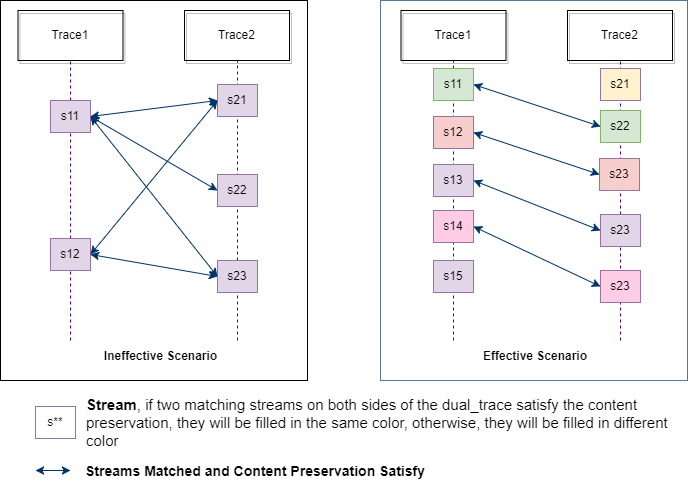
\includegraphics[scale=0.55]{Figures/secondlevelmatching}}
 \caption{Second Level Matching Scenarios}
\label{secondlevelmatching}
\end{figure}


The following subsections of this one discuss the algorithms for these two level matching. In Section\ref{windows}, I elaborate the channel open process and the data transfer categories for the concerned communication methods. Based on the different channel process, two algorithms are developed for first level matching, one is for Named Pipe and Message Queue, while the other is for TCP and UDP. The input of the first level algorithm is the two endpoint lists of the two traces of the analyzing dual-trace while the output is the identified channels. Each channel contains the matched endpoints from both side of the traces. The data transfer characteristics divided the communication methods into reliable and unreliable transmissions. Named pipe and TCP fall in the reliable category while MSMQ and UDP fall in the unreliable one. The second level matching algorithms are distinct for these two categories. The corresponding second level data matching algorithms are being used in the first level algorithms. The input of the second level algorithms is the streams of both endpoint while the output a boolean to indicate if the transmitted data of this two endpoint streams are matched.

\subsection{Communication Identification Algorithm for Named pipe and Message Queue}
For the Named pipe and MSMQ only one channel open function is being call for each endpoint. So in the below algorithm, when it try to get the channel open event from the $endpoint.openStream$ list, only one event should be found and return. The channel identifier parameters can be found in the $event.inputs$ of the channel open event. The identifier for Named pipe is the file name of the pipe while for MSMQ is the format queue name of the queue. 

This algorithm will find out all the possible channels regardless some of them might be false positive. The called data verification algorithm should be ``Matching by Data Streams Algorithm" for Named pipe and ``Matching by Data Events Algorithm" for MSMQ.

\begin{algorithm}[H]
\DontPrintSemicolon
\caption{{\bf Communication Indentification Algorithm for Named pipe and Message Queue} \label{channelAlg1}}
\KwIn{two endpoint lists of the dual-trace}
\KwOut{communication list}
$communications \leftarrow Map \langle String, List \langle Communication \rangle \rangle$;\; 
\For{$endpoint1 \in endpointList1$}{
   $openEvent1 \leftarrow$ get the event from $endpoint1.openStream$, which should only contain one event;\;
   $channelId1 \leftarrow$ get the channel identifier from $openEvent1.inputs$;\;
   \For{$endpoint2 \in endpointList2$}{
      $openEvent2 \leftarrow$ get the event from $endpoint2.openStream$, which should only contain one event;\;
      $channelId2 \leftarrow$ get the channel identifier from $openEvent2.inputs$;\;
     \If{$channelId1 == channelId2$}{
         $DataVerified  \leftarrow $ Call the corresponding data verification algorithm.
         \If{$DataVerified == True$}{
            $communication = New \enspace Communication()$;\;
            $communication.endpoint1 = endpoint1$;\;
            $communication.endpoint2 = endpoint2$;\;
            $communication.dataMatch\leftarrow$ The output from data verification algorithm;\;
            $communications.add\left( communication \right)$;\;
         }    
      }
   }
}
\KwRet $channels$;\;
\end{algorithm} 


\subsection{Communication Identification Algorithm for TCP and UDP}
For TCP and UDP multiple functions are collaborating to create the final communication channel. Local address and port of the server endpoint and Remote address and port of the client endpoint are used to identify the channel. This algorithm first try to get the Local address and port of the server endpoint and remote address and port from client endpoint. Then it try to match two endpoints by comparing the local and remote address and port.

\begin{algorithm}[H]
\DontPrintSemicolon
\caption{{\bf Communication Indentification Algorithm for TCP and UDP} \label{channelAlg2}}
\KwIn{two endpoint lists of the dual-trace}
\KwOut{channel list}
$communications \leftarrow Map \langle String, List \langle Communication \rangle \rangle$;\; 
\For{$endpoint1 \in endpointList1$}{
   $bindEvent1 \leftarrow$ get the $bind\left( \right)$ function call related event from $endpoint1.openStream$;\;
   $connectEvent1 \leftarrow$ get the $connect\left( \right)$ function call related event from $endpoint1.openStream$;\;
   \For{$endpoint2 \in endpointList2$}{
      $bindEvent2 \leftarrow$ get the $bind\left( \right)$ function call related event from $endpoint2.openStream$;\;
      $connectEvent2 \leftarrow$ get the $connect\left( \right)$  function call related event from $endpoint2.openStream$;\;
    \If{$socketEvent1 !=null$ AND $socketEvent2 != null$}{
       \If{$bindEvent1 != null$ AND $connectEvent2 == null$}{
           $localServerAddr \leftarrow$ get the serverAddr parameter value from $bindEvent1.inputs$;\;
       }
       \ElseIf{$bindEvent2 == null$ AND $connectEvent1 != null$}{
           $remoteServerAddr \leftarrow$ get the serverAddr parameter value from $connectEvent1.inputs$;\; 
       }
       \Else{
          Break the inner For loop;\;
       }
       \If{$localServerAddr == remoteServerAddr$}{
          $DataVerified  \leftarrow $ Call the corresponding data verification algorithm.
          $communication = New \enspace Communication()$;\;
          $communication.endpoint1 = endpoint1$;\;
          $communication.endpoint2 = endpoint2$;\;
          $communication.dataMatch\leftarrow$ The output from data verification algorithm;\;
          $communications.add\left( communication \right)$;\;
       }
    }
   }
}
\KwRet $channels$;\;
\end{algorithm}

\subsection{Transmitted Data Verification for Named pipe and TCP by Data Union}
As describe in Section\ref{reliable} the data being receive by one endpoint should always equal to or at least is sub string of the data being sent fro the other endpoint in a communication for the reliable transmission methods, such as Named pipe and TCP. So the transmitted data verification algorithm is in data union level. The send data union is retrieved by the conjunction of the input buffer content of the send events in the send stream of an endpoint. The receive data union is retrieved by the conjunction of the output buffer content of the receive events in the receive stream of an endpoint. The input of this algorithm is the two endpoints from two traces which are being matched.
\begin{algorithm}[H]
\DontPrintSemicolon
\caption{{\bf Transmitted Verification by Data Union} \label{dataAlg1}}
\KwIn{two endpoint from each trace of the dual-trace}
\KwOut{send data union and receive data union of two endpoints}
\KwRet{Indicator of if transmitted data union are considered to be identical}
$send1 \leftarrow$ empty string;\;
$send2 \leftarrow$ empty string;\;
$recv1 \leftarrow$ empty string;\;
$recv2 \leftarrow$ empty string;\;
\For{$sendEvent \in endpoint1.sendStream$}{
   $sendmessage \leftarrow$ get the input buffer content from the $sendEvent.inputs$;\;
   $send1.append\left( sendmessage \right)$;\;
}
\For{$sendEvent \in endpoint2.sendStream$}{
   $sendmessage \leftarrow$ get the input buffer content from the $sendEvent.inputs$;\;
   $send2.append\left( sendmessage \right)$;\;
}
\For{$recvEvent \in endpoint1.receiveStream$}{
   $recvmessage \leftarrow$ get the output buffer content from the $recvEvent.outputs$;\;
   $recv1.append\left( sendmessage \right)$;\;
}
\For{$recvEvent \in endpoint2.receiveStream$}{
   $recvmessage \leftarrow$ get the output buffer content from the $recvEvent.outputs$;\;
   $recv2.append\left( sendmessage \right)$;\;
}
\If{$recv1$ is substring of $send2$ AND $recv2$ is substring of $send1$ }{
   \KwRet True;\;
}
\Else{
    \KwRet False;\;
}

\end{algorithm} 

\subsection{Transmitted Data Verification for MSMQ and UDP by Data of Events}
For the unreliable communication methods, the data packets being transmitted are not delivery and ordering guaranteed. So it is impossible to verify the transmitted data as a whole chunk. Fortunately, the packets arrived to the receivers are always as the original one from the sender. Therefore, we perform the transmitted data verification by single events instead of the whole stream. This algorithm basically goes through the send event list from one endpoint trying to find the matched receive event from the receive event list from the other endpoint. And then calculate the fail packet arrival rate. The fail packet arrival rate should be comparable to the packet lost rate. So we set the packet lost rate as the threshold to determine if the transmitted data can considered to be identical in both directions. The packet lost rate can be various from network to network or even from time to time for the same network. The inputs of this algorithm are the copies of two endpoints from two traces which are being matched, the packet lost rate as the threshold. The threshold should be an integer. For example if the lost rate is 5\%, the threshold should be set as 5. I use copies instead of original endpoints is that for efficiency I modify the input list directly in the algorithm.
\begin{algorithm}[H]
\DontPrintSemicolon
\caption{{\bf Transmitted Verification by Data of Events } \label{dataAlg2}}
\KwIn{two endpoint lists of the dual-trace, threshold}
\KwOut{matched event list of two endpoints}
\KwRet{Indicator of if transmitted data union are considered to be identical}
$sendPktNum1 \leftarrow endpoint1.sendStream.length$;\;
$sendPktNum2 \leftarrow endpoint2.sendStream.length$;\;
$recvPktNum1 \leftarrow 0$;\;
$recvPktNum2 \leftarrow 0$;\;
$eventMatchs \leftarrow List \langle EventMatch \rangle$;\;
\For{$sendEvent \in endpoint1.sendStream$}{
   $sendmessage \leftarrow$ get the input buffer content from the $sendEvent.inputs$;\;
   \For{$recvEvent \in endpoint2.receiveStream$}{
      $recvmessage \leftarrow$ get the output buffer content from the $recvEvent.outputs$;\;
      \If{$sendmessage == recvmessage$}{
         $recvPktNum1++$;\;
         $endpoint2.receiveStream.remove\left( recvEvent \right)$;\;
         $eventMatch = New eventMatch\left( \right)$;\;
         $eventMatchs.add\left( eventMatch \right)$;\;
      }
   }
}

\If{$ \left(sendPktNum1-recvPktNum1\right)*100/sendPktNum1 > threshold$}{
 \KwRet False;\;
}

\For{$sendEvent \in endpoint2.sendStream$}{
   $sendmessage \leftarrow$ get the input buffer content from the $sendEvent.inputs$;\;
   \For{$recvEvent \in endpoint1.receiveStream$}{
      $recvmessage \leftarrow$ get the output buffer content from the $recvEvent.outputs$;\;
      \If{$sendmessage == recvmessage$}{
         $recvPktNum2++$;\;
         $endpoint1.receiveStream.remove\left( recvEvent \right)$;\;
      }
   }
}

\If{$ \left(sendPktNum2-recvPktNum2\right)*100/sendPktNum2 > threshold$}{
 \KwRet False;\;
}
 \KwRet True;\;
\end{algorithm}



\section{Data Structures for Identified Communications}
In the previous sections, I elaborate all the essential algorithms to identify the communications. The information of identified communications should be organized properly for the further presentation or visualization to the user. In this section, I define the output data structures to fulfill this requirement. There are totally two major data structure. The first one is clustered as communications align the definition at Section\ref{definition}. The second one is clustered by endpoints in the traces. The reason to provide the second data structure is due to the false positive errors of the channel identification. The endpoint lists in the traces provides more original data information. So with other assistant information and the access of the relatively original information from the dual-trace, the user has more flexibility to analysis the dual-trace. This data structures have been used in the algorithms implicitly.

\begin{algorithm}[H]
\DontPrintSemicolon
\caption{{\bf Data Structure for Identified Communications} \label{communicationlData}}
$communications \leftarrow Map \langle String, List \langle Communication \rangle \rangle$;\tcp*[f]{communication clustering}\;  
$traceEndpoints \leftarrow Map \langle String, List \langle Endpoint \rangle \rangle$; \tcp*[f]{endpoint clustering}\;  
\Struct{Communication}{
  Endpoint endpoint1 \tcp*[f]{endpoint1 is from trace1 of the dual-trace}\;  
  Endpoint endpoint2 \tcp*[f]{endpoint2 is from trace2 of the dual-trace}\;  
  DataMatch dataMatch\;  
}

\Struct{Endpoint}{
  Int \quad \quad handle\;
  Stream \enspace stream\;
}

\Union{DataMatch}{
  DataUnionMatch \quad  unionMatch \tcp*[f]{For data union verification}\;  
  List $\langle$ EventMatch $\rangle$ \enspace eventMatchs \tcp*[f]{For data event verification}\;  
}

\Struct{DataUnionMatch}{
  String sData1 \tcp*[f]{send data union of endpoint1}\;  
  String rData1 \tcp*[f]{receive data union of endpoint1,substring of sData2}\;  
  String sData2 \tcp*[f]{send data union of endpoint2}\;  
  String rData2 \tcp*[f]{receive data union of endpoint2,substring of sData1}\; 
}

\Struct{EventMatch}{
  Event \quad \quad event1 \tcp*[f]{event1 is from enpoint1}\;  
  Event \quad \quad event2 \tcp*[f]{event2 is from enpoint2}\;  
}


\Struct{Stream}{
  List $\langle$ Event $\rangle$ \enspace openStream\;
  List $\langle$ Event $\rangle$ \enspace closeStream\;
  List $\langle$ Event $\rangle$ \enspace sendStream\;
  List $\langle$ Event $\rangle$ \enspace receiveStream\; 
}

\Struct{Event}{
   Int \quad \quad \quad \quad \quad \quad \quad \quad lineNum\;
   Map $\langle$ String, String $\rangle$ \enspace inputs\; 
   Map $\langle$ String, String $\rangle$ \enspace outputs\; 
}

\end{algorithm} 